\chapter{Introduction}
\label{cha:Introduction}

\begin{figure}
    \centering
    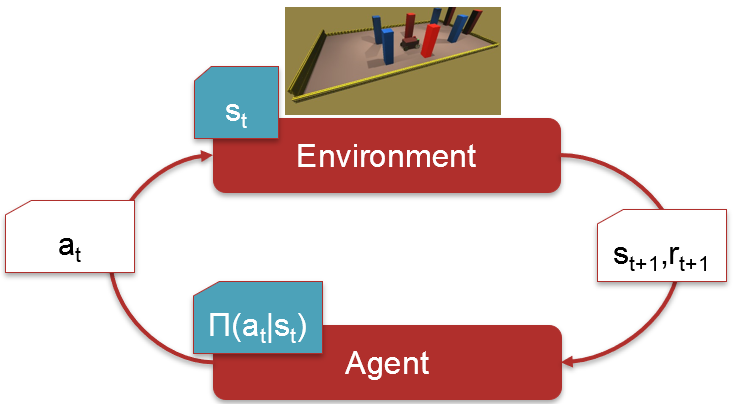
\includegraphics[width=0.8\textwidth]{Bilder/rl_cycle.png}
    \caption{Loop in Collect Data}
    \label{fig:unitycommunication}
\end{figure}


\renewcommand{\thepseudonum}{\roman{pseudonum}}
\begin{pseudocode}{Train Model}{ }
\COMMENT{Sample from replay buffer and update the model based on the loss}\\

\PROCEDURE{TrainModel}{}
amount\_of\_batches \GETS \frac{rollout\_buffer\_size}{batch\_size}\\
\FOR i \GETS 0 \TO n\_epochs \DO
\BEGIN
RolloutBuffer.\CALL{Shuffle}{}\\
\FOR i \GETS m \TO amount\_of\_batches \DO
\BEGIN
batch \GETS RolloutBuffer.\CALL{GetBatch}{m}\\
loss \GETS \CALL{ComputeLoss}{batch}\\
Model.\CALL{Backpropagate}{loss}\\
Optimizer.\CALL{Step}{}\\
\END\\
\END
\ENDPROCEDURE

\end{pseudocode}
